%
% idee.tex -- Polynom Idee
%
\section{Idee
\label{reedsolomon:section:idee}}
\rhead{Problemstellung}
Um Fehler in einer Datenübertragung zu erkennen, könnte man die Daten jeweils doppelt senden,
    also immer zwei gleich Werte miteinander und so jeweils einzelne Fehler erkennen.
Wenn jedoch mehr als nur ein Fehler erkannt werden soll und sogar noch das Orginal rekonstruiert werden soll,
dann werden die Daten drei oder vierfach versendet.
Doch nur schon um Fehler zu erkennen werden überproportional viele Daten doppelt und dreifach gesendet.
Das Problem liegt darin Informationen, Zahlen, 
    zu Übertragen und Fehler zu erkennen und zu korrigieren.
Der Unterschied des Fehler Erkennens und Korrigirens, ist das beim Erkennen nur die Frage beantwortet wird: Ist die Übertragung fehlerhaft oder nicht?
Beim Korrigieren werden Fehler erkannt und dann zusätzlich noch die Originalwerte rekonstruiert.
Eine weitere Möglichkeit wäre, dass der Empfänger nach einer fehlerhaften Übertragung die selben Daten nochmals anfordert.
Dies führt wieder zu unerwünschten mehrfachen Übertragung.
In Anwendungen des Reed-Solomon-Codes Abschnitt \externaldocument{papers/reedsolomon/anwendungen} \ref{reedsolomon:section:anwendung}
    ist diese vom Empfänger gesteuerte erneute Übertragen meistens nicht sinnvoll oder sogar unmöglich.
Der Reed-Solomon-Code macht dies Übertragung auf eine andere, clevere Weise.

\subsection{Polynom-Ansatz
\label{reedsolomon:section:polynomansatz}}
\rhead{Polynom-Ansatz}
Eine zentrale Idee des Reed-Solomon-Code ist, aus den Daten ein Polynom zu bilden. 
Von dieser Polynomfunktion wird dann eine Anzahl Werte übertragen.
\begin{beispiel} Nehmen wir die Zahlen \textcolor{blue}{2}, \textcolor{blue}{1}, \textcolor{blue}{5},
    welche übertragen werden sollen. Daraus bilden wir das Polynom
\begin{equation}
p(x)
=
\textcolor{blue}{2}x^2 + \textcolor{blue}{1}x + \textcolor{blue}{5}
\label{reedsolomon:equation1}
\end{equation}.
\par 
Ein Polynome zweiten Grades ist durch drei Punkte eindeutig bestimmbar. 
Bei einer fehlerlosen Übertragung können wir mit 3 übertragene Werte
    das Polynom durch Polynominterpolation volständig rekonstruieren.
Wir brauchen Polynominterpolation als Methode, um aus Punkte wieder Polynom zu berechnen.
Die Koeffizente des rekonstruierten Polynoms sind dann unsere gesendeten Zahlen \textcolor{blue}{2}, \textcolor{blue}{1}, \textcolor{blue}{5}.
\par 
Wie können wir nun Fehler erkennen oder sogar korrigieren?
Versuchen wir doch mehr Werte zu übertragen, wir nehmen im Beispiel 7 Werte.
Übertragen werden nun die \textcolor{darkgreen}{grünen Werte} 
    dieses \textcolor{blue}{blauen Polynomes} an den Stellen 1, 2, 3, \dots , 7.
In Abbildung \ref{fig:polynom} ist das zu den \textcolor{blue}{Datenpunkten} gehörige Polynom blau dargestellt,
    die \textcolor{darkgreen}{übertragenen Werte} des Polynoms sind grün.
Die grünen Punkte bestimmen die Parabel. 
Damit können die Fehler erkannt werden, weil die empfangenen Punkte nicht auf der Parabel liegen.
Somit können die grauen Punkte auf der Parabel ersetzt werden und sind damit korrigiert.
Bis zu wievielen Fehler können wir nun im Beispiel korrigieren?
Wir erhöhen nun die Fehleranzahl Schritt für Schritt:
\begin{itemize}
    \item[\textit{1 Fehler}:] Bei einem Fehler können konkurrenzierende, aber falsche Polynome zusammen mit zwei originalen Punkten entstehen.
        Dabei können aber maximal 3 Punkte auf diesem Konkurrenzpolynom sein.
        Da 6 > 3 ist haben wir unser original Polynom gefunden.
    \item[\textit{2 Fehler}:] Bei Zwei Fehlern kann ein Fehler mit zwei originalen Punkten ein konkurrenzierendes, aber falsches Polynom bilden.
        Da der zweite \textcolor{red}{Fehler} frei wählbar ist, kann dieser auch auf dem \textcolor{gray}{Konkurrenzpolynom} liegen, wie in der Abbilbung \ref{fig:polynom}.
        Nun haben wir, ein \textcolor{blue}{originales Polynom} mit \textcolor{darkgreen}{5} übereinstimmenden und eine konkurrenzierendes mit 4 Punkten.
        Da 5 noch grösser als 4 ist, können wir sagen, welches das Originalpolynom ist.
    \item[\textit{3 Fehler}:] Bei Drei kann genau wie bei 2 oder 1 Fehler, ein konkurenzierendes Polynom mit einem Fehler und zwei originalen Punkten bestimmen werden.
        Auch hier sind die anderen Fehler frei wählbar und liegen auf dem Konkurrenzpolynom.
        Nun ist es so das 5 Punkte auf diesem konkurenzierenden Polynom und 4 Punkte auf dem originalen.
        Das Originalpolynom kann nicht mehr gefunden werden.
    \item[\textit{4 Fehler}:] Bei Vier, kann es noch erkannt werden, dass Fehler statt gefunden haben, da 3 orginale Punkte das ursprüngliche Polynom ergeben.
        Somit haben wir mindestens 2 verschieden Polynome, dass bedeutet Fehler sind entstanden.
    \item[\textit{5 Fehler}] Bei Fünf, kann mit den 2 originalen Punkte das Originale Polynom nicht mehr erkannt werden und 
        somit auch keine Aussgae gemacht werden ob Fehler statt gefunden haben oder nicht.
\end{itemize}

\begin{figure}%[!ht]
	\centering
	%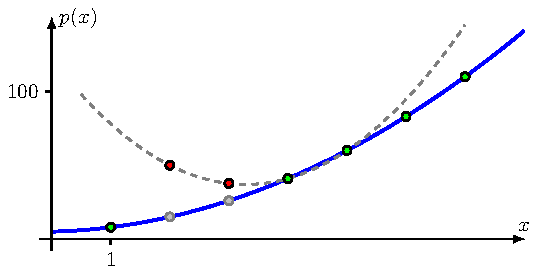
\includegraphics[width=\textwidth]{papers/reedsolomon/figures/polynom2}
    % polynomraw

\newcommand{\teiler}{40}


%//////////////////////////////////////

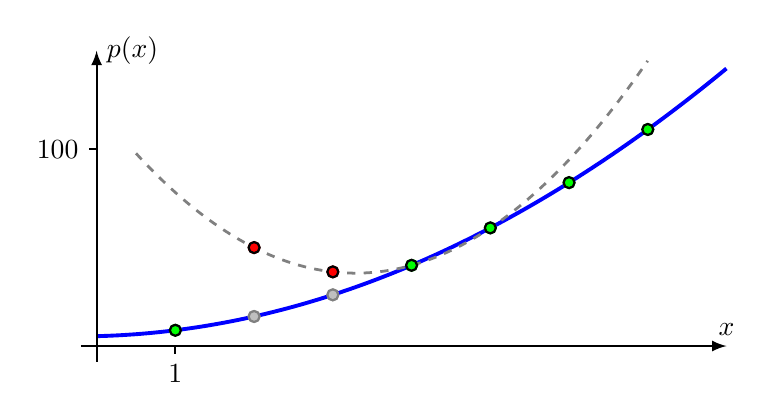
\begin{tikzpicture}[>=latex,thick,]
	\draw[color=blue, line width=1.4pt] 
	plot[domain=0:8, samples=100]
	({\x},{(2*\x^2+1*\x+5)/\teiler});

	\draw[->] (-0.2,0) -- (8,0) coordinate[label={$x$}];
	\draw[->] (0,-0.2) -- (0,150/\teiler) coordinate[label={right:$p(x)$}];
	
	\def\punkt#1{
		\fill[color=green] #1 circle[radius=0.08];
		\draw #1 circle[radius=0.07];
	}

	\def\hellpunkt#1{
		\fill[color=lightgray] #1 circle[radius=0.08];
		\draw[gray] #1 circle[ radius=0.07];
	}
	
	\draw[color=gray,line width=1pt,dashed] 
	plot[domain=0.5:7, samples=100]
	({\x},{(7.832*\x^2-51.5*\x+121.668)/\teiler});


	\punkt{(1,8/\teiler)}
	\hellpunkt{(2,15/\teiler)}
	\hellpunkt{(3,26/\teiler)}
	\punkt{(4,41/\teiler)}
	\punkt{(5,60/\teiler)}
	\punkt{(6,83/\teiler)}
	\punkt{(7,110/\teiler)}
	

	
	\def\erpunkt#1{
		\fill[color=red] #1 circle[radius=0.08];
		\draw #1 circle[radius=0.07];
	}
	\erpunkt{(2,50/\teiler)}
	\erpunkt{(3,37.66/\teiler)}

	\draw(0,100/\teiler) -- (-0.1,100/\teiler) coordinate[label={left:$100$}];
	\draw(1,0) -- (1,-0.1) coordinate[label={below:$1$}];		
\end{tikzpicture}
	\caption{Polynom $p(x)$ von der Gleichung\eqref{reedsolomon:equation1}}
	\label{fig:polynom}
\end{figure}
\qedhere
\end{beispiel}

\section{Anzahl Übertragungswerte bestimmen
\label{reedsolomon:section:Fehlerkorrekturstellen}}
Um zu bestimmen, wieviel zusätzliche \textcolor{darkgreen}{Übertragungspunkte} notwendig sind, um die Fehler zu korrigieren,
    muss man zuerst wissen, wieviel \textcolor{blue}{Datenwerte} gesendet und wieviel \textcolor{red}{Fehler} erkennt werden sollen. 
Die Anzahl Datenwerte, ergeben die Anzahl Polynomkoeffizente \textcolor{blue}{$k$} und somit den Grad $k-1$.
Die Bestimmung der Anzahl der Fehler \textcolor{red}{$t$}, welche korrigiert werden können, braucht Redundanz.
Gehen wir die Fehleranzahl mit verschiedenen Übertragungsanzahlen durch, 
    erkennt man almählich ein Muster.
\begin{table}%[!ht]
    \centering
    \begin{tabular}{ c c | c} 
        \hline
        Nutzlas & Fehler & Übertragen \\
        \hline 
        3 & 2 & 7 Werte eines Polynoms vom Grad 2 \\ 
        4 & 2 & 8 Werte eines Polynoms vom Grad 3 \\
        3 & 3 & 9 Werte eines Polynoms vom Grad 2 \\ 
        \hline
        $k$ & $t$ & $k+2t$ Werte eines Polynoms vom Grad $k-1$ \\ 
        \hline
    \end{tabular}
    \caption{ Fehlerkorrekturstellen Bestimmung.}
    \label{tab:fehlerkorrekturstellen}
\end{table}
\par 
Es müssen mehr Punkte auf dem \textcolor{blue}{originalen Polynom} liegen, als auf dem konkurenzierenden.
Somit braucht man für die Übertragung pro \textcolor{red}{Fehler} zwei Übertragungspunkte mehr.
Wie in der Tabelle ergibt sich diese \textcolor{darkgreen}{Übertragungsanzahl}
\begin{equation}
    \textcolor{darkgreen}{u}=
    \textcolor{blue}{k}+2\textcolor{red}{t}.
    \label{reedsolomon:equation2}
\end{equation}

Ein Nebeneffekt ist, dass auch $2t$ Fehler erkannt werden können, nicht aber korrigiert.
Für die Polynomkoeffizente nach der Übertragung zu rekonstruieren, 
    haben wir jedes mal die Polynominterpolationmethode angewendet.
Diese Polynoiminterpolation ist leider schwierig und fehleranfällig.
Deshalb finden wir eine alternative im nächsten Abschnitt.

